\documentclass[20pt,landscape]{foils}
\usepackage[pdftex]{color}
\usepackage[pdftex]{graphicx}
\usepackage[pdftex]{geometry}
\geometry{headsep=2ex,hscale=0.9} \pdfpagewidth=11in
\pdfpageheight=8.5in

\setlength{\footskip}{0.0in} \setlength{\textheight}{8.0in}

\usepackage{background}
\usepackage{pp4slide}
%\usepackage{pdfscreen}


\newtheorem{lemma}{Lemma}

\newcommand{\br}{{\mathbf r}}
\newcommand{\bA}{{\mathbf A}}
\newcommand{\ba}{{\bf a}}
\newcommand{\bb}{{\bf b}}
\newcommand{\bd}{{\bf d}}
\newcommand{\bs}{{\bf s}}
\newcommand{\bbm}{{\bf m}}
\newcommand{\bn}{{\bf n}}
\newcommand{\bv}{{\bf v}}
\newcommand{\bw}{{\bf w}}
\newcommand{\bbf}{{\bf f}}
\newcommand{\bC}{{\bf C}}
\newcommand{\bE}{{\bf E}}
\newcommand{\bF}{{\bf F}}
\newcommand{\bG}{{\bf G}}
\newcommand{\bH}{{\bf H}}
\newcommand{\bS}{{\bf S}}
\newcommand{\bT}{{\bf T}}
\newcommand{\bN}{{\bf N}}
\newcommand{\bD}{{\bf D}}
\newcommand{\bX}{{\bf X}}
\newcommand{\bP}{{\bf P}}
\newcommand{\bI}{{\bf I}}
\newcommand{\bR}{{\bf R}}
\newcommand{\bU}{{\bf U}}
\newcommand{\bV}{{\bf V}}
\newcommand{\bW}{{\bf W}}
\newcommand{\bJ}{{\bf J}}
\newcommand{\bB}{{\bf B}}
% \newcommand{\bcS}{{\bf {\cal S}}}
% \newcommand{\bcH}{{\bf {\cal H}}}
\newcommand{\bzero}{{\bf 0}}
\newcommand{\bgamma}{{\mbox {\boldmath $\gamma$}}}
\newcommand{\btheta}{{\mbox {\boldmath $\theta$}}}
\newcommand{\bLambda}{{\mbox {\boldmath $\Lambda$}}}
\newcommand{\bPsi}{{\mbox {\boldmath $\Psi$}}}
\newcommand{\bPhi}{{\mbox {\boldmath $\Phi$}}}
\newcommand{\bcS}{{\mbox {\boldmath ${\cal S}$}}}
\newcommand{\bcH}{{\mbox {\boldmath ${\cal H}$}}}
\newcommand{\bcI}{{\mbox {\boldmath ${\cal I}$}}}
\newcommand{\bcR}{{\mbox {\boldmath ${\cal R}$}}}
\newcommand{\bcB}{{\mbox {\boldmath ${\cal B}$}}}

\begin{document}

\raggedright \color{white}
%\definecolor{bgcolor}{rgb}{1,1,1}
\definecolor{bgcolor}{rgb}{0.0,0.0,0.0}
\pagecolor{bgcolor} % set background color
\definecolor{bgblue}{rgb}{0.04,0.37,0.59}
\vpagecolor{bgblue}

%%---------Cover Page
\foilhead{\LARGE Multiuser Receiver Design Maximizing Mutual
Information Rate}
\begin{center}
\vspace{.3in}
{\bf Hanhong Shen }  \\
{\it \vspace{0.5in} Wireless System Research Laboratory \\Dept. of Electrical \& Computer Engineering \\
\& Computer Science \\ Cincinnati,
OH~~45221-0030} \\
\vspace{.5in}
\end{center}

%%----- Slide  1
\foilhead{\LARGE Multi-Access Interference (MAI)}
\begin{itemize}
\item In TDMA systems (GSM and IS136), MAI comes from overlapping
slots originating in other cells and from users in the same cell
due to channel dispersion.

\item In orthogonal CDMA systems (IS95 and CDMA2000), the
orthogonality can not be guaranteed at each receiver once they go
through the channel. Especially in asynchronous case. MAI is hard
to be avoided even in the absence of channel distortion or
other-cell interference.

\item In FDMA systems (AMPS), extra guard bands have to be used to
separate different users.

\item In some other MIMO system, such as OFDM and DMT, MAI can
appear as ISI or cross talk.
\end{itemize}

%%--------Slide 2
\foilhead{\LARGE Multiuser Detection}
\begin{itemize}
\item Multiuser detection refers to data detection in
non-orthogonal multiplexes.

\item The MAI has considerable structure and much less randomness
than the white Gaussian background noise.

\item By exploiting this structure, multiuser detection can
increase spectral efficiency, receiver sensitivity and the number
of substantiable users. It can also reduce the reliance on tight
and accurate power control.

\item Multiuser detection comes in various flavors.

    \begin{itemize}
    \item Optimal: jointly and individually optimal multiuser
    detection.
    \item Linear: decorrelating detection, MMSE detection and MAME detection.
    \item Nonlinear: hard interference cancellations.
    \end{itemize}

\end{itemize}

%%-------- Slide 3
\foilhead{\LARGE Multiuser Channel Model}
\begin{center}
\vspace{-0.5in}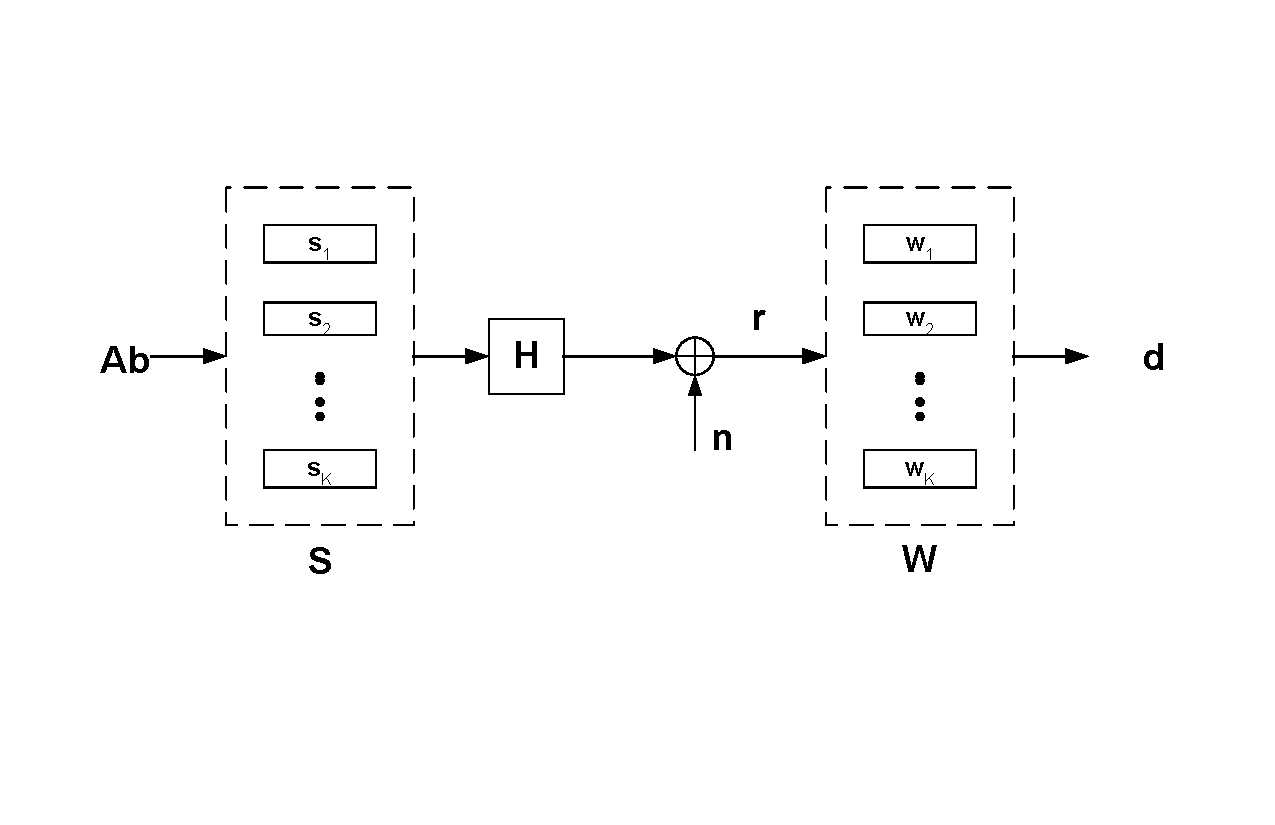
\includegraphics[width=7in]{MIMO_channel.pdf}
\end{center}
where $\br=\bH\bS\bA\bb+\bn$ and $\bd=\bW^T\bH\bS\bA\bb+\bW^T\bn$.
For the sake of simplification, $\bH$ is set to be $\bI$ in the
following.

%--------Slide 4
\foilhead{\LARGE Multiuser Receiver Design Criteria I}
\begin{itemize}
\item Minimum bit-error rate (BER). Individually and jointly
optimum multiuser receivers.

$$\bw_k^{IO} = \mbox{arg}\min_{\bw}P_e^{IO}\mbox{  and  }\bW^{JO} =
\mbox{arg}\min_{\bW}P_e^{JO}$$

\item Decorrelating detector (DD), which minimizes MAI.

$$\bW^{DD} = \bS^{+}$$

\item Minimum mean-square errors (MMSE) receiver.

$$\bW^{MMSE}=\bS(\bS^{T}\bS^{}+\sigma^2\bA^{-2})^{-1}$$

\end{itemize}

%% ------- slide 5
\foilhead{\LARGE Multiuser Receiver Design Criteria II}
\begin{itemize}
\item Maximum asymptotical multiuser efficiency (MAME) receiver.

$$\bw_k^{MAME}=\mbox{arg}\max_{\bw}\eta_k$$

\item Decision-driven multiuser detector. (hard interference
cancellation)

$$\hat{b}_k=\mbox{sgn}\left\{\bs_k^T(\br-\mbox{Est. MAI})\right\}$$

\item Maximum mutual information rate (MMIR) receiver. (my topic)

$$\bW^{MMIR}=\mbox{arg}\max_{\bW}\bI(\bb;\ \bd)$$

\end{itemize}

%--------Slide 6
\foilhead{\LARGE Mutual Information Rate I}

The mutual information per input symbol between any input block
$\bb$ of $K$ users/channels and the corresponding output block
$\bd$ of $M$ receivers is maximized when the additive noise $\bbm$
is Gaussian and is given by (N. Al-Dhahir and J. M. Cioffi, 1996)

$$\begin{array}{rcl} \bI(\bb;\ \bd)&=& {1\over
K}\log_2\left|(\bR_b^{+}+\bG\bR_m^{-1}\bG^H)\bR_b\right|
\end{array}$$

\begin{itemize}
\item $\bd =\bG^H\bb+\bbm$ and $\bb$ are the output/input of a
MIMO system.

\item $\bb$ and $\bbm$ are zero-mean independent vectors with
covariance matrices $\bR_b$ and $\bR_m$. And $\bbm$ is additive
Gaussian noise.
\end{itemize}

%% ------- slide 7
\foilhead{\LARGE Mutual Information Rate II}

\begin{itemize}

\item It shows that $\bI(\bb;\ \bd)$ is maximized when the
eigenvectors of $\bR_b$ are matched to those of
$\bG\bR_m^{-1}\bG^H$. (Hadamard inequality)

\item The choice of $\bG$ effects the mutual information rate of
the blocks though MIMO channel.

\item The choice of $\bG$ is not unique. When $\bbm=\bG^H\bn$,
$\bG$ can be written as $\bU\bF$, where $\bn$ is AWGN vector,
$\bU$ is the eigenvector matrix of $\bR_b$ and $\bF$ can be any
compatible and invertible matrix.
\end{itemize}

%% ----- slide 8
\foilhead{\LARGE MMIR Multiuser Receiver}

\begin{itemize}

\item $\bW^{MMIR}=\bU\bF$, where $\bU$ is the eigenvector matrix
of $\bS\bS^T$ and $\bF$ is any invertible $L\times K$ matrix.

\item The final output is
$\hat{\bb}=\mbox{sgn}\{\bF^T\bU^T\bS\bA\bb+\bF^T\bU^T\bn\}$ \item
The maximization of multiuser channel capacity can't guarantee the
minimization of final BERs.

\item The choice of $\bF$ can greatly effect the performance of
MMIR multiuser receivers.
\end{itemize}

%% ------------ Slide 9
\foilhead{\LARGE The Choice of $\bF$}

\begin{itemize}
\item When $\bF=\bE$, where $\bE=\bU^T\bS$, $\bW^{MMIR}$ is equal
to $\bS$ and single-user matched filter is one of the solutions to
maximize $\bI(\bb;\ \bd)$.

\item When $\bF=\bE\bR_s^{-1}=\bR_s^{-1/2}$, where
$\bR_s=\bS^T\bS$, $\bW^{MMIR}$ is equal to $\bW^{DD}$ and
decorrelating detector is one of the solutions to maximize
$\bI(\bb;\ \bd)$, too.

\item When $\bF=\bE(\bR_s+\sigma^2\bI)^{-1}$, $\bW^{MMIR}$ becomes
$\bW^{MMSE}$ and MMSE detector also is one of the solutions to
maximize $\bI(\bb;\ \bd)$.

\item What about other possible choices?
\end{itemize}

%% ----------- Slide 10
\foilhead{\LARGE Computer Simulations}
\begin{center}
\vspace{-1.0in}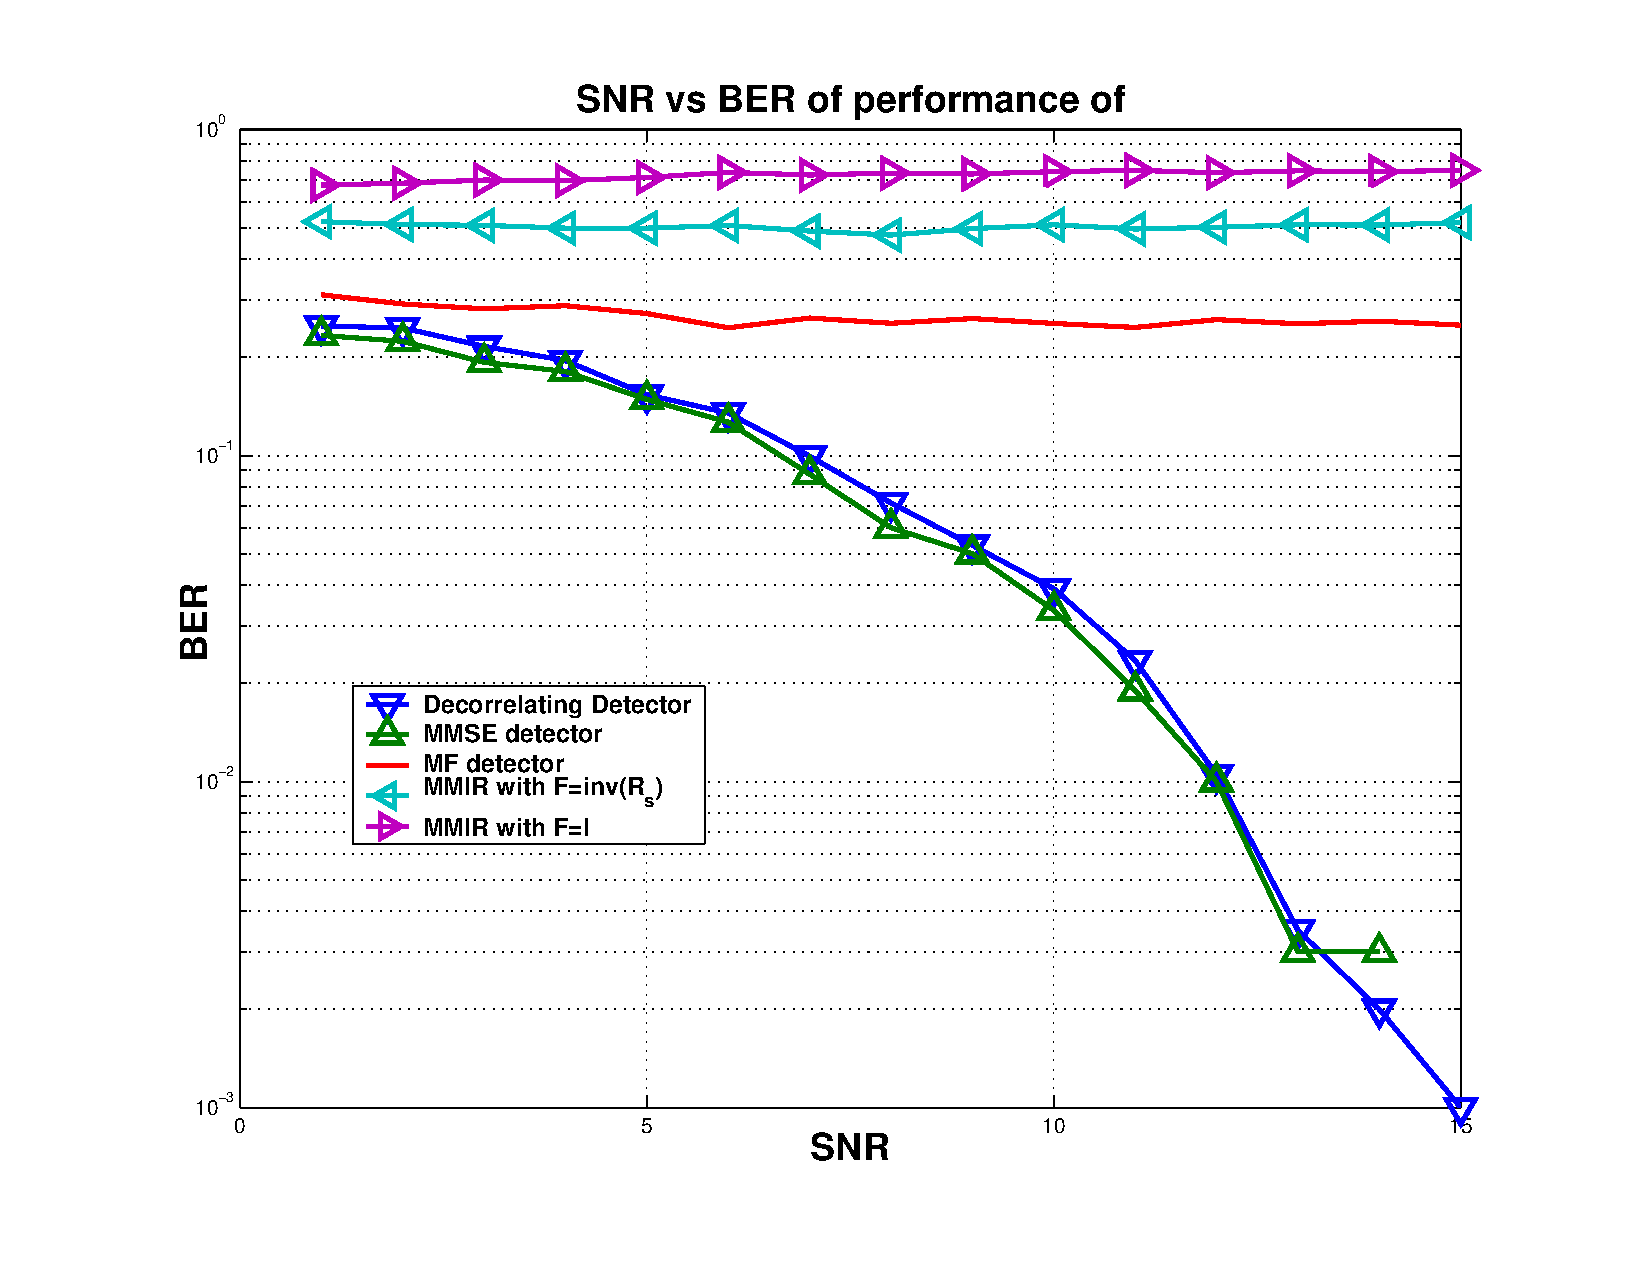
\includegraphics[width=8in]{SNR.pdf}
\end{center}


%% ----------- Slide 11
\foilhead{\LARGE Blind MMIR Multiuser Receiver}

\begin{itemize}
\item
Autocorrelation matrix of the receiver signal $\br$ is given by
(X. Wang and H. V. Poor, 1998)
$$\bR_r=\mbox{E}\{\br\br^T\}=\bS\bA^2\bS^T+\sigma^2\bI=\bU\bar\bLambda\bU^T$$
where $\bU=\left[\matrix{\bU_s&\bU_n}\right]$ and
$\bar\bLambda=\left[\matrix{\bar\bLambda_s&\mathbf{0}\cr\mathbf{0}&\bar\bLambda_n}\right]=\bA^2+\sigma^2\bI$.

\item Blind $\bW^{DD}$ can be expressed as
$\bU_s(\bar\bLambda_s-\sigma^2\bI)^{-1}\bU_s^T\bS$. Blind
$\bW^{MMSE}$ can be expressed as
$\bU_s\bar\bLambda_s^{-1}\bU_s^T\bS$ \item Blind $\bW^{MMIR}$ can
also be easily constructed if $\bF$ is available.
\end{itemize}

%% ---------------- Slide 12
\foilhead{\LARGE Computer Simulations I}
\begin{center}
\vspace{-1.0in}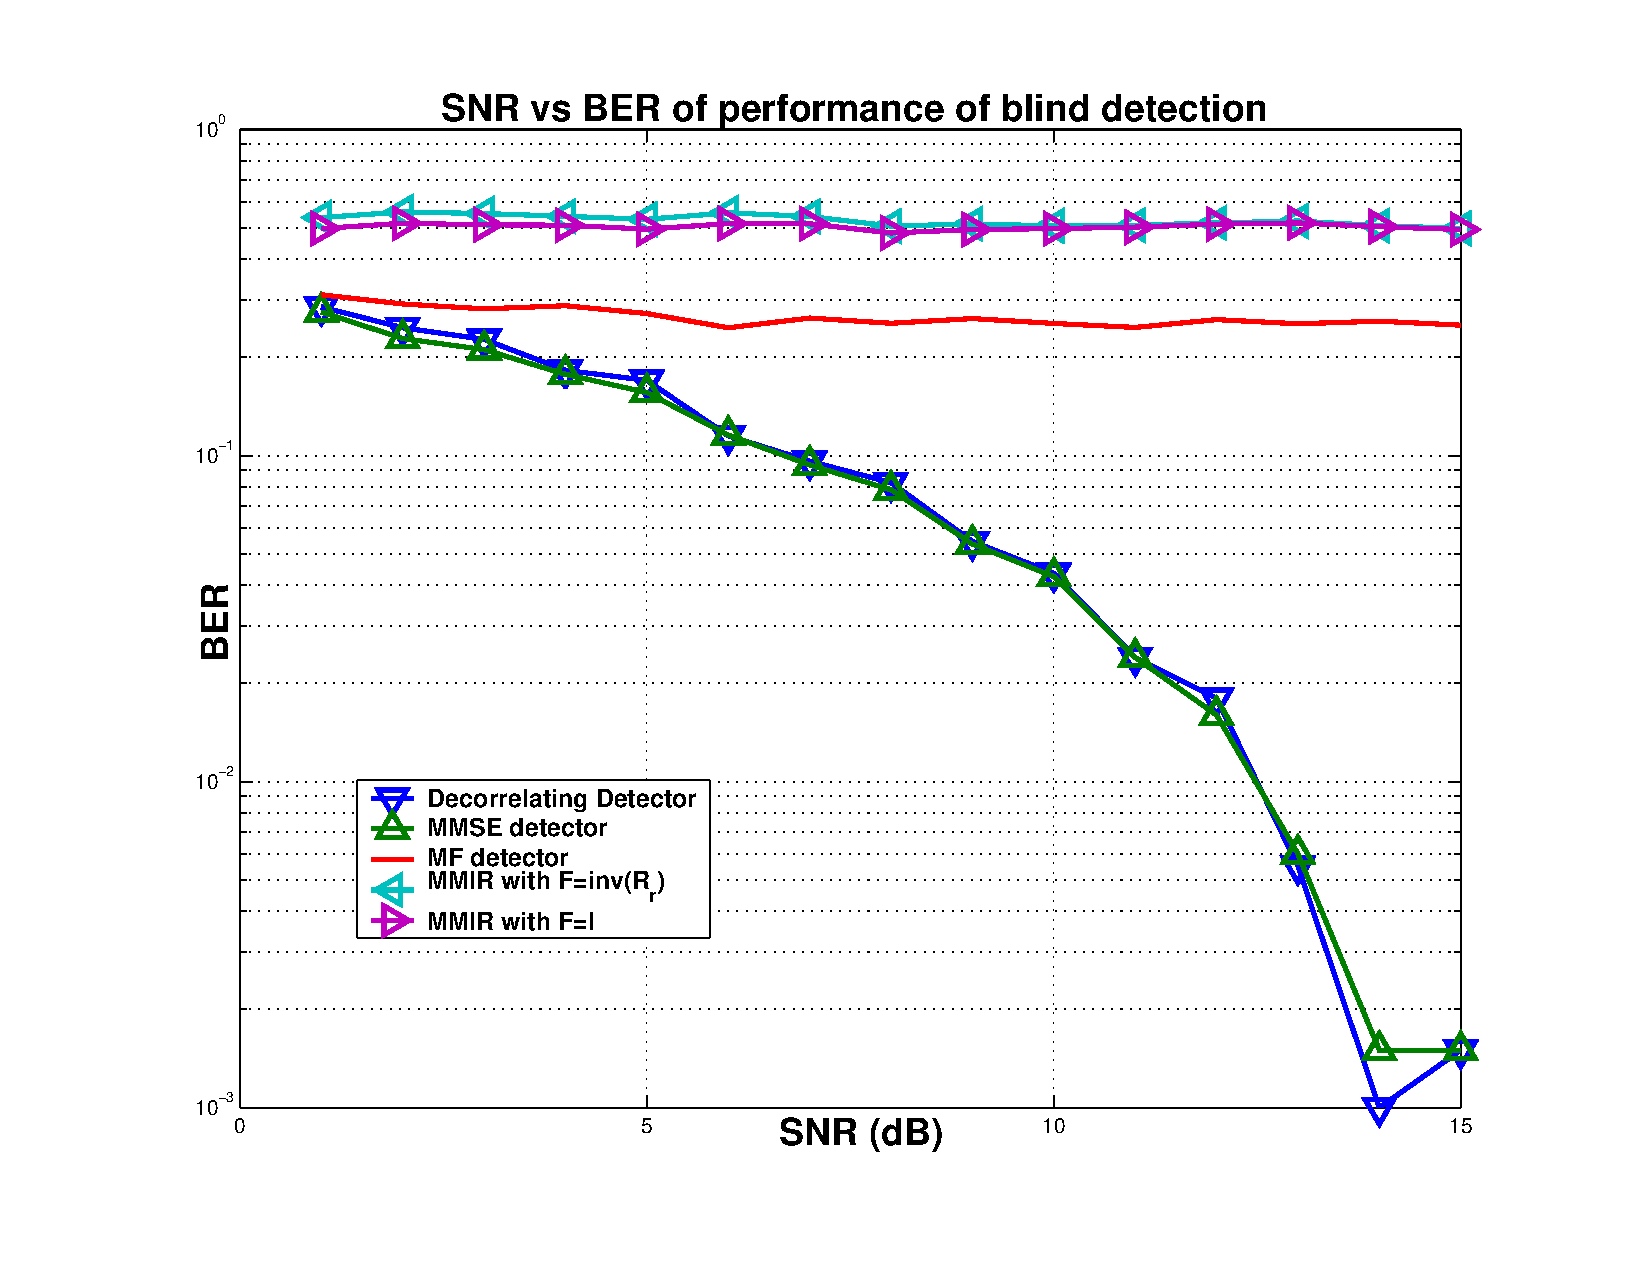
\includegraphics[width=8in]{BlindSNR.pdf}
\end{center}

\foilhead{\LARGE Computer Simulations II}
\begin{center}
\vspace{-1.0in}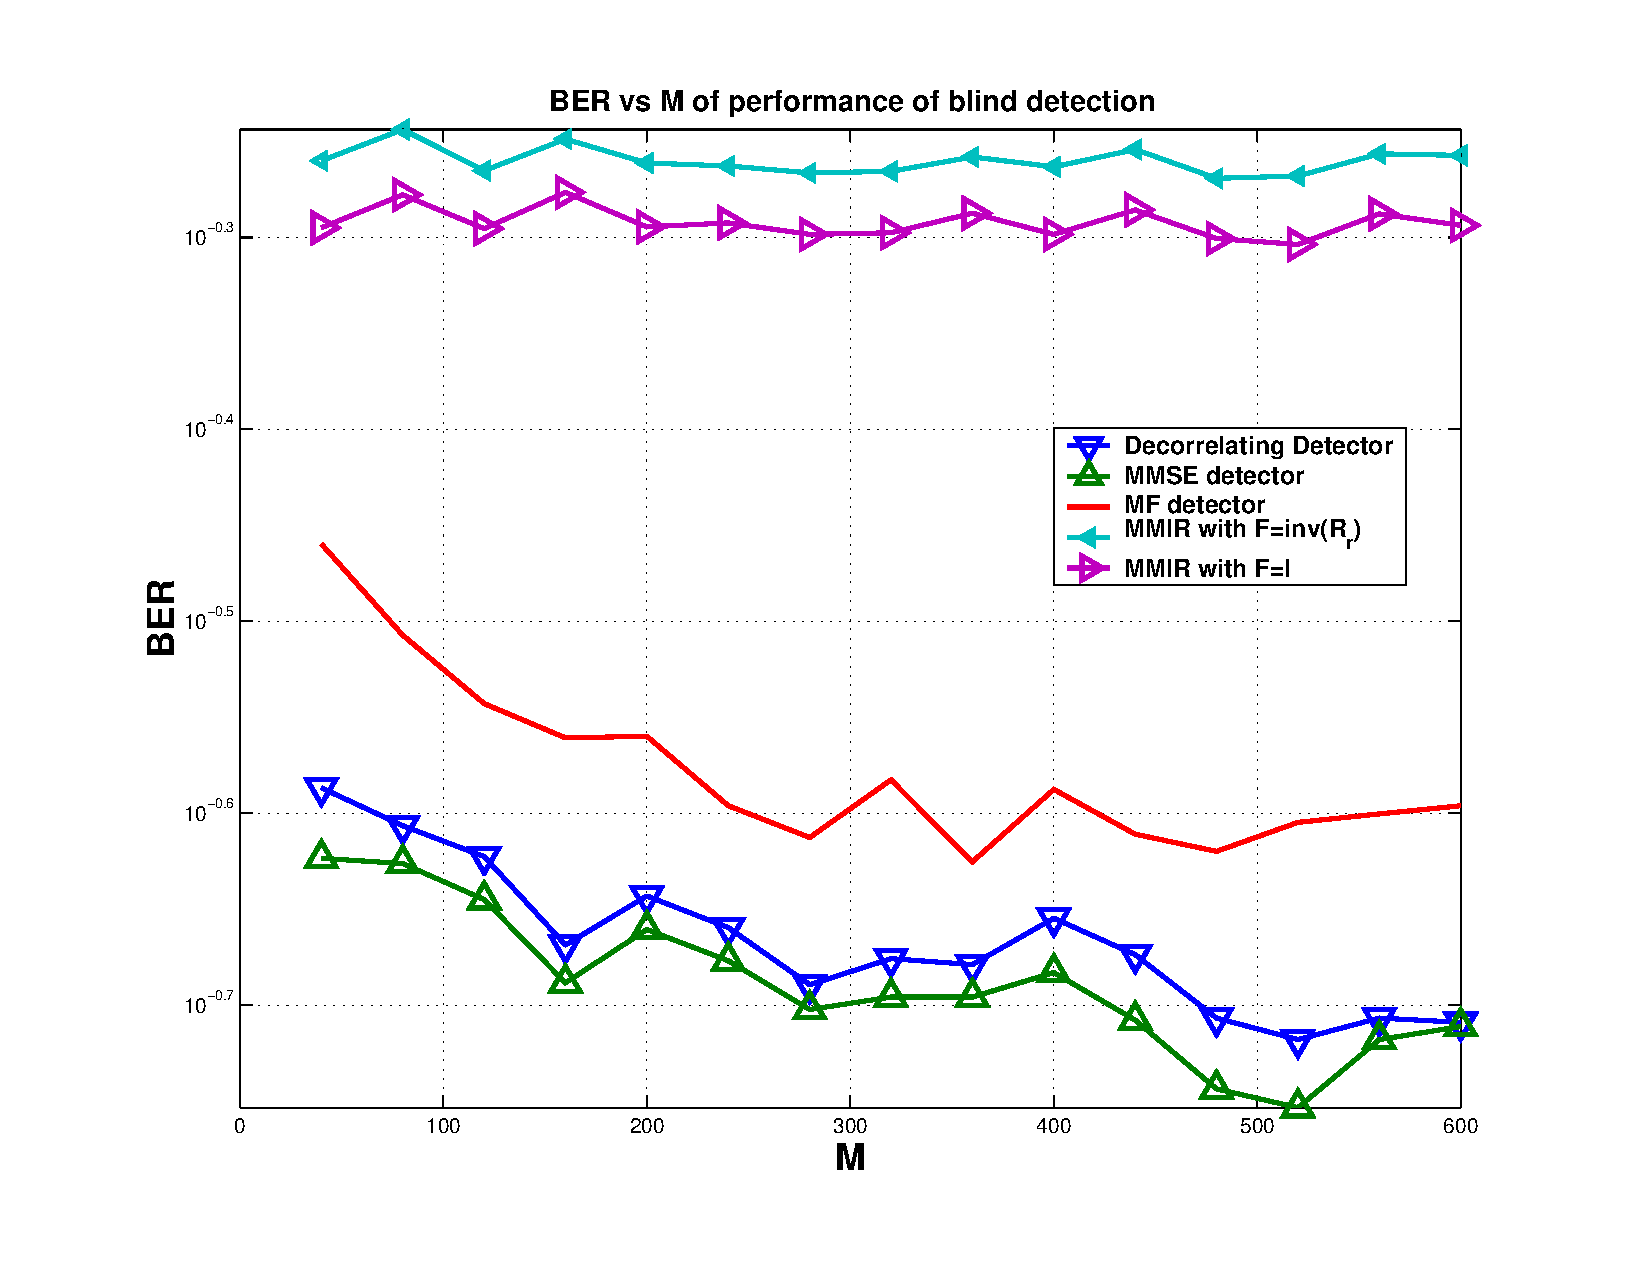
\includegraphics[width=8in]{M.pdf}
\end{center}
%% -------------- Slide 13
\foilhead{\LARGE Conclusions \& Future Directions}

\begin{itemize}
\item It is interesting to find that many existing multiuser
detectors satisfy the proposed MMIR constrain.

\item Multiuser receiver can not be completely decided only by
MMIR constrain. Additional constrain is needed. In the future, it
is very important to look for additional constrain to decide
$\bF$.

\item It is also very interesting to look for adaptive realization
of blind MMIR receiver.

\item Since the model is the basic MIMO system model, many
previous discussions are applicable in many other MIMO systems,
such as OFDM, DMT and multi-antenna system.
\end{itemize}


%% -------- Slide 14
\foilhead{\LARGE Selected References}

\begin{itemize}
\item \small Naofal Al-Dhahir and John M. Cioffi, Block
Transmission over Dispersive Channels: Transmit Filter
Optimization and Realization, and MMSE-DFE Receiver Performance,
IEEE Transactions On Information Theory, Vol. 42, January 1996,
pp. 137-160.

\item Anna Scaglione, S. Barbarossa and G. B. Giannakis,
Filterbank transceivers optimizing information rate in block
transmissions over dispersive channels, IEEE Transactions On
Information Theory, Vol. 3, April 1999, pp. 1019 -1032.

\item Xiaodong Wang and H. Vincent Poor, Blind Multiuser
Detection: A Subspace Approach, IEEE Transaction On Information
Theory, Vol. 44, No. 2, March 1998, pp.677-690.
\end{itemize}

\end{document}
